\documentclass[main.tex]{subfiles}
\begin{document}


\section{Hogere orde afgeleiden}
\label{sec:hogere-orde-afgel}

\begin{de}
  Beschouw een functie $f:\ A \subseteq \mathbb{R} \rightarrow \mathbb{R}$.
  Stel dat $A$ enkel ophopingspunten bevat.
  Noteer de verzamelingen van punten van $A$ waarin $f$ afleidbaar is als $A_{1}$.
  Noteer bovendien met $f':\ A_{1} \rightarrow \mathbb{R}:\ x \mapsto f'(x)$ de afgeleide functie van $f$.

  Zij $a$ een element van $A$, dan noemen we $f$ \term{twee maal afleidbaar} in $a$ als en slechts als $a$ tot $A_{1}$ behoort, een ophopingspunt is van $A_{1}$ en de afgeleide functie $f'$ afleidbaar is in $a$.
  We noteren de \term{tweede orde afgeleide} functie $(f')'$ van $f$ als $f''$.
  We noemen $f$ \term{twee maal afleidbaar} op $A$ als $f$ twee maal afleidbaar is in elke $a\in A$.
\end{de}

\begin{st}
  \label{st:berekening-tweede-afgeleide}
  Als de tweede afgeleide van een functie $f$ in een punt $a$ bestaat, dan kunnen we ze als volgt berekenen:
  \[ f''(x) = \lim_{h \rightarrow 0}\frac{f(x+h)+f(x-h)-2f(x)}{h^{2}} \]

  \begin{proof}
    \[ 
    \begin{array}{rl}
      f''(x)
      &= \lim_{h \rightarrow 0}\frac{f'(x+h)-f'(x)}{h}\\
      &= \lim_{h \rightarrow 0}\frac{\lim_{h \rightarrow 0}\frac{f(x+h)-f(x+h-h)}{h}-\lim_{h \rightarrow 0}\frac{f(x)-f(x-h)}{h}}{h}\\
      &= \lim_{h \rightarrow 0}\frac{\lim_{h \rightarrow 0}\frac{f(x+h)-f(x+h-h)-f(x)+f(x-h)}{h}}{h}\\
      &= \lim_{h \rightarrow 0}\frac{\lim_{h \rightarrow 0}\frac{f(x+h)-2f(x)+f(x-h)}{h}}{h}\\
      &= \lim_{h \rightarrow 0}\frac{f(x+h)+f(x-h)-2f(x)}{h^{2}} \\
    \end{array}
    \]
    \question{waarom mogen we zomaar dezelfde $h$ gebruiken?}
    \question{Mogen we zomaar de andere definitie van een afgeleide gebruiken?}
  \end{proof}
\end{st}

\begin{de}
  Zij $I$ een interval in $\mathbb{R}$ dan noemen we $C(I)$ de verzameling van continue functies van $I$ naar $\mathbb{R}$.
  Voor $n\in \mathbb{N}$ noemen we $C^{n}(I)$ de verzameling van continue functies die $n$ keer afleidbaar zijn op $I$ en waarvoor $f^{(n)}$ continu is op $I$.
  Met $C^{\infty}(I)$ noteren we de verzameling van functies $I$ die onbeperkt afleidbaar zijn op $I$.
\end{de}

\begin{st}
  Zij $I$ een interval in $\mathbb{R}$, voor elke $n\in \mathbb{N}$ is $C^{n}(I)$ een vectorruimte.
\extra{bewijs}
\end{st}

\begin{st}
  Zij $I$ een interval in $\mathbb{R}$, voor elke $n\in \mathbb{N}$ is $C^{n}(I)$ gesloten onder het product:
  \[ \forall f,g \in C^{n}(I):\ fg \in C^{n}(I) \]
\extra{bewijs}
\end{st}


\begin{vb}
  Beschouw de functie $f:\ \mathbb{R} \rightarrow \mathbb{R}:\ x \mapsto |x|x^{4}$.
  \extra{hoeveel keer is $f$ afleidbaar?}
\end{vb}

\begin{de}
  \label{de:convexe-functie}
  Zij $f:\ I \subseteq \mathbb{R} \rightarrow \mathbb{R}$ een functie gedefinieerd op een interval $I$, dan noemen we $f$ \term{convex} over een deelinterval $I_{0}$ van $I$ als en slechts als het volgende geldt:
  \[ \forall x,y \in I_{0}, \forall \lambda \in \interval{0}{1}:\ f((1-\lambda)x+\lambda y) \le (1-\lambda)f(x) + \lambda f(y)\]
\end{de}
\begin{de}
  We noemen $f$ \term{concaaf} over $I_{0}$ als en slechts als $-f$ convex is.
\end{de}

\begin{opm}
  Een functie kan zowel convex als concaaf zijn.
  $f: x \mapsto 0$ bijvoorbeeld.
\end{opm}

\begin{bpr}
  Beschouw een functie $f:\ I \subseteq \mathbb{R} \rightarrow \mathbb{R}$, gedefinieerd op een open interval $I$ die twee keer afleidbaar is.
  $f$ is convex over $I$ als en slechts als $f''$ positief is over heel $I$.

  \begin{proof}
    Bewijs van een equivalentie
    \begin{itemize}
    \item $\Rightarrow$\\
      Zij $f$ een convexe functie.
      Kies een willekeurige $x\in I$.
      Omdat $I$ open is, bestaat er een $\delta \in \mathbb{R}_{0}^{+}$ zodat $\interval[open]{x-\delta}{x+\delta}$ een deel is van $I$.
      Omdat $f$ convex is, gelden de volgende twee ongelijkheden voor alle $h \in \interval[open]{-\delta}{\delta}$:
      (Kies $\lambda = \frac{1}{2}$ in de definitie van convexiteit\deref{de:convexe-functie})
      \[ f\left(\frac{1}{2}(x-h) + \frac{1}{2}(x+h)\right) \le \frac{1}{2}f(x-h) + \frac{1}{2}f(x+h) \]
      \[ f(x) \le \frac{1}{2}f(x-h) + \frac{1}{2}f(x+h) \]
      \[ 2f(x) \le f(x-h) + f(x+h) \]
      \[ f(x-h) + f(x+h) -2f(x) \ge 0 \]
      \[ \frac{f(x+h)+f(x-h)-2f(x)}{h^{2}} \ge 0 \]
      Nemen we nu de limiet van deze ongelijkheid voor $h$ gaande naar nul, dan krijgen we het volgende\prref{pr:limiet-behoudt-orde}:
      \[ \lim_{h \rightarrow 0}\frac{f(x+h)+f(x-h)-2f(x)}{h^{2}} \ge \lim_{h \rightarrow 0}0 \]
      \[ f''(x) \ge 0 \]
      $f''$ is positief in een willekeurige $x$\stref{st:berekening-tweede-afgeleide} en dus over heel $I$.
    \item $\Leftarrow$\\
      Zij $f$ een functie zodat $f''$ positief is over een open interval $I$
      Kies willekeurig $x,y \in I$   met $x < y$ en $\lambda \in \interval{0}{1}$.
      Voor $\lambda = 0$ of $\lambda = 1$ is dit deel triviaal.
      Stel daarom dat $\lambda \in \interval[open]{0}{1}$ geldt en noteer $z = (1-\lambda)x + \lambda y$.
      Volgens de middelwaardestelling van Lagrange bestaan er dan $c_{x}\in \interval[open]{x}{z}$ en $c_{y}\in \interval[open]{z}{y}$ als volgt\stref{st:middelwaardestelling-lagrange}:
      \[ f'(c_{x}) = \frac{f(z)-f(x)}{z-x} \quad\text{ en }\quad f'(c_{y}) = \frac{f(y)-f(z)}{y-z} \]
      We kunnen nu $f(z)$ uitwerken:
      \[
      \begin{array}{rl}
        f(z) 
        &= (1-\lambda)f(z) + \lambda f(z)\\
        &= (1-\lambda)\left((z-x)f'(c_{x}) + f(x)\right) - \lambda\left( f'(c_{y})(y-z)-f(y)\right)\\
        &= (1-\lambda)f(x) + \lambda f(y) + (1-\lambda)(z-x)f'(c_{x}) + \lambda(z-y)f'(c_{y})\\
        &= (1-\lambda)f(x) + \lambda f(y) + \lambda(1-\lambda)(y-x)(f'(c_{x})-f'(c_{y}))\\
      \end{array}
      \]
      \question{hoe gebeurt die laatste stap?}
      Gebruiken we nu de middelwaardestelling van Lagrange, dan vinden we een $c \in \interval{c_{x}}{c_{y}}$ als volgt:\stref{st:middelwaardestelling-lagrange}
      \[ f''(c) = \frac{f'(c_{y})-f'(c_{x})}{c_{y}-c_{x}} \]
      Gaan we nu verder met de vorige gelijkheid, dan vinden we de volgende ongelijkheid, waar uit volgt dat $f$ convex is over $I$.
      \[ 
      \begin{array}{rl}
        f(z) &= (1-\lambda)f(x) + \lambda f(y) + \lambda(1-\lambda)(y-x)(f'(c_{x})-f'(c_{y}))\\
             &= (1-\lambda)f(x) + \lambda f(y) + \lambda(1-\lambda)(y-x)f''(c)(c_{y}-c_{x})\\
             &\le (1-\lambda)f(x) + \lambda f(y) 
      \end{array}
      \]
      In de laatste ongelijkheid gebruiken we $f''(c) \ge 0$, $y > x$, $c_{y}> c_{x}$ en $\lambda(1-\lambda) \ge 0$.
    \end{itemize}
  \end{proof}
\end{bpr}


\section{Middelwaardestelling van Taylor}
\label{sec:midd-van-tayl}

\begin{bst}
  \label{st:middelwaardestelling-taylor}
  Beschouw een functie $f:\ I \subseteq \mathbb{R} \rightarrow \mathbb{R}$, gedefinieerd op een interval $I$, die $n$ maal afleidbaar is op $I$ en $(n+1)$ maal op het inwendige $\mathring{I}$ van $I$.
  Stel dat $f^{(n)}$ continu is op $I$ en zij $a,x\in I$ met $a \neq x$, dan bestaat er een $c$, strikt tussen $a$ en $x$, als volgt:
  \[ 
  f(x) = \frac{f^{(n+1)}(c)}{(n+1)!}(x-a)^{n+1} + \sum_{n = 0}^{n}\frac{f^{(n)}(a)}{n!}(x-a)^{n} 
  \]
  \TODO{bewijs p 43}

  \begin{proof}
    Definieer $R$ als volgt:
    \[ R = f(x) -  \sum_{n = 0}^{n}\frac{f^{(n)}(a)}{n!}(x-a)^{n}  \]
    We tonen aan dat er een $c\in \interval[open]{a}{x}$ bestaat als volgt:
    \[ R = \frac{f^{(n+1)}(c)}{(n+1)!}(x-a)^{n+1} \]
    Definieer bovendien een funcie $F:\ I \rightarrow \mathbb{R}$ als volgt:
    \[ F(t) = \sum_{n = 0}^{n}\frac{f^{(n)}(t)}{n!}(x-t)^{n} + R\frac{(x-t)^{n+1}}{(x-a)^{n+1}} \]
    Merk op dat $F(x)$ gelijk is aan $f(x)$ en bovendien $F(a) = f(x)$ geldt.
    $F$ is continu op $I$ en afleidbaar op $\mathring{I}$ \waarom
    Bovendien geldt ziet $F'$ er als volgt uit:
    \[
    \begin{array}{rl}
      F'(t)
      &= \sum_{n = 0}^{n}\frac{f^{(n)}(t)}{n!}(x-t)^{n} + R\frac{(x-t)^{n+1}}{(x-a)^{n+1}} \\
      &= \sum_{n = 0}^{n}\left(\frac{f^{(n+1)}(t)}{n!}(x-t)^{n} - \frac{f^{(n)}(t)}{n!}n(x-t)^{n}\right)+  R(n+1)\frac{(x-t)^{n}}{(x-a)^{n+1}}\\
      &= \frac{f^{(n+1)}(t)}{n!}(x-t)^{n} - R(n+1)\frac{(x-t)^{n}}{(x-a)^{n+1}}\\
    \end{array}
    \]
    We kunnen nu op $F$ en $\interval[open]{a}{x}$ de middelwaardestelling van Rolle toepassen.\stref{st:rolle}
    Er bestaat dus een $c$, strikt tussen $a$ en $x$ zodat $c$ een nulpunt is van $F'(c)$:
    \[ 0 = F'(c) = \frac{f^{(n+1)}(c)}{n!}(x-c)^{n} - R(n+1)\frac{(x-c)^{n}}{(x-a)^{n+1}} \]
    Omdat $c$ verschillend is van $x$ vinden we $R$ als volgt:
    \[ R = \frac{(x-a)^{n+1}}{n+1}\frac{f^{(n+1)}(c)}{n!} = \frac{f^{(n+1)}(c)}{(n+1)!}(x-a)^{n+1} \]
    \extra{wat betekent dit bewijs...}
  \end{proof}
\end{bst}

\begin{opm}
  Merk op dat de middelwaardestelling van Lagrange hier eigenlijk een speciaal geval van is.
  Namelijk wanneer $n$ $1$ is.
\end{opm}

\begin{de}
  Beschouw een functie $f:\ I \subseteq \mathbb{R} \rightarrow \mathbb{R}$, gedefinieerd op een interval $I$, die $n$ maal afleidbaar is op $I$ en $(n+1)$ maal op het inwendige $\mathring{I}$ van $I$.
  Stel dat $f^{(n)}$ continu is op $I$ en zij $a,x\in I$ met $a \neq x$, dan noemen we $P_{n}$ als volgt de \term{$n$-de orde benadering} van $f$ rond $a$.
  \[ 
  P_{n}(x) = \sum_{n = 0}^{n}\frac{f^{(n)}(a)}{n!}(x-a)^{n} 
  \]
  We noemen deze veelterm soms de \term{Taylorveelterm} van graad $n$ van $f$ rond $a$.
  In bovenstaande stelling noemen we de eerste term de \term{restterm} van graad $n$ en we noteren deze als $R_{n}(x)$.
  \[ 
  R_{n}(x) = \frac{f^{(n+1)}(c)}{(n+1)!}(x-a)^{n+1} 
  \]
\end{de}

\begin{de}
  We noemen het rechterlid als volgt de \term{Taylor(reeks)ontwikkeling} van $f$ rond $a$ in $x$.
  \[
  f(x) = \lim_{n \rightarrow \infty}\sum_{n = 0}^{n}\frac{f^{(n)}(a)}{n!}(x-a)^{n} 
  \]
\end{de}

\begin{st}
  Beschouw een $n$-degraads veeltermfunctie $f:\ \mathbb{R} \rightarrow \mathbb{R}$ en $a\in \mathbb{R}$.
  Voor elke $x\in A$ kan $f(x)$ uitgedrukt worden in termen van de afgeleiden van $f$ in $a$ als volgt:
  \[ 
  f(x) = \sum_{n = 0}^{n+1}\frac{f^{(n)}(a)}{n!}(x-a)^{n} 
  \]
  \begin{proof}
    Zij $f:\ \mathbb{R} \rightarrow \mathbb{R}$ een $n$-degraads veeltermfunctie een $a\in \mathbb{R}$, $f$ is onbeperkt afleidbaar.\needed
    Vanaf de $n+2$-e afgeleide is $f^{(n)}$ overal nul voor alle $n\in \mathbb{N}$.
    Volgens de stelling van Taylor bestaat er een $c\in\interval[open]{x}{a}$ als volgt:\stref{st:middelwaardestelling-taylor}
    \[ f(x) = \frac{f^{(n+2)}(c)}{(n+2)!}(x-a)^{n+2} + \sum_{n = 0}^{n+1}\frac{f^{(n)}(a)}{n!}(x-a)^{n} \]
    We weten echter dat $f^{(n+2)}(c)$ nul moet zijn, en bekomen zo de stelling:
    \[ f(x) = 0 + \sum_{n = 0}^{n+1}\frac{f^{(n)}(a)}{n!}(x-a)^{n} \]
  \end{proof}
\end{st}

\begin{vb}
  Beschouw de functie $f$:
  \[ f:\ \mathbb{R} \setminus \{1\} \rightarrow \mathbb{R}:\ x \mapsto \frac{1}{1-x} \]
  Kies $a=0$.
  Beschouw nu de afgeleiden van $f$:
  \[ \forall k\in \mathbb{N}, \forall x\in \mathbb{R}\setminus\{1\}:\ f^{(k)}(x) = \frac{k!}{(1-x)^{k+1}} \]
  Er geldt steeds $f^{(k)}(a) = f^{(k)}(0) = k!$.
  Passen we nu de stelling van Taylor toe, dan krijgen we het volgende:\stref{st:middelwaardestelling-taylor} 
  \[ \forall x\in \interval[open]{-\infty}{1},\ \exists c:\ \frac{1}{1-x} = \sum_{k=0}^{n}x^{k} + \frac{x^{n+1}}{(1-c)^{n+2}} \]
  We bekijken nu de restterm $R_{n}$:
  \[ R_{n} = \frac{x^{n+1}}{(1-c)^{n+2}} = \frac{1}{1-x}-\sum_{k=0}^{n}x^{k} = \frac{1-x^{n+1}}{1-x} = \frac{x^{n+1}}{1-x} \]
  We zien dat de limiet van $R_{n}$ voor $n$ gaande naar $+\infty$ inderdaad nul is voor $|x|<1$.
  We vinden dus de volgende reeksontwikkeling voor $f$ rond $0$ voor alle $x\in \interval[open]{-1}{1}$:
  \[ \frac{1}{1-x} = \lim_{n \rightarrow +\infty}\sum_{k=0}^{n}x^{k} \]
  \begin{figure}[H]
    \centering
    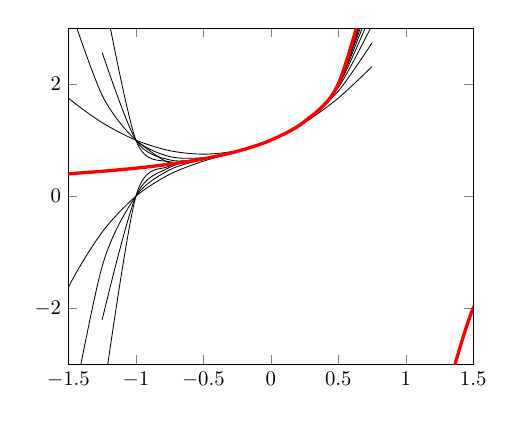
\begin{tikzpicture}[scale=.75]
      \begin{axis}[xmin=-1.5, xmax=1.5, ymin=-3,ymax=3, restrict y to domain=-5:5]
        \foreach \n in {2,...,10}{
          \addplot[smooth,domain=-2:4]{1/(1-x)-(x^(\n+1))/(1-x)};
        }
        \addplot[smooth,domain=-2:4,color=red,ultra thick]{1/(1-x)};
      \end{axis}
    \end{tikzpicture}
  \end{figure}
\end{vb}

\begin{vb}
  Beschouw de functie $f$:
  \[ 
  f:\ \mathbb{R} \rightarrow \mathbb{R}:\ x \mapsto 
  \left\{
    \begin{array}{rl}
      e^{-\frac{1}{x^{2}}} & \text{ als } x \neq 0\\
      0 & \text{ als } x = 0\\
    \end{array}
  \right.
  \]
  Kies $a=0$.
  $f$ is onbeperkt afleidbaar op $\mathbb{R}_{0}$.
  Bovendien zien de afgeleiden er als volgt uit:
  \[ \forall k\in \mathbb{N}:\ f^{(k)}(x) = e^{-\frac{1}{x^{2}}}q_{k}\left(\frac{1}{k}\right) \]
  Hierin is $q_{k}$ een veeltermfunctie van graad $3k$.
  Ook in $0$ is $f$ onbeperkt afleidbaar met afgeleide telkens nul.
  $f$ heeft echter \textbf{geen} Taylorreeksontwikkeling rond $0$ voor om het even welke $x \neq 0$. 
\end{vb}

\begin{de}
  We noemen een functie $f:\ A \subseteq \mathbb{R} \rightarrow \mathbb{R}$, gedefinieerd op een open deel $A$ van $\mathbb{R}$, \term{analytisch} op $A$ als er voor elke $a\in A$ een $\delta \in \mathbb{R}_{0}^{+}$ bestaat als volgt:
  \begin{itemize}
  \item $\interval[open]{a-\delta}{a+\delta} \subseteq A$
  \item Er bestaat een rij $(c_{n})_{n}$ in $\mathbb{R}$ zodat voor alle $\interval[open]{a-\delta}{a+\delta}$ het volgende geldt:
    \[ f(x) = \lim_{n\rightarrow +\infty}\sum_{k=0}^{n}c_{k}(x-a)^{k} \]  
  \end{itemize}
\end{de}

\begin{bpr}
  Zij $f:\ I \subseteq \mathbb{R} \rightarrow \mathbb{R}$ een twee maal afleidbare functie op een open interval $I$ zodat de tweede afgeleide $f''$ continu is.
  Stel dat er een nulpunt $a\in I$ van $f'$ bestaat, dan geldt het volgende:
  \begin{itemize}
  \item Als $f''$ strikt positief is in $a$, dan bereikt $f$ in $a$ een lokaal minimum.
  \item Als $f''$ strikt negatief is in $a$, dan bereikt $f$ in $a$ een lokaal maximum.
  \end{itemize}

  \begin{proof}
    \begin{idee}
      Het lokaal minimum/maximum ligt in een lokaal 'kuiltje'.
      We zoeken dat kuiltje via de tweede afgeleide en bewijzen door het bestaan ervan het bestaan van het lokaal maximum/minimum.
    \end{idee}
    
    Omdat $f''$ continu is, kunnen we een $\delta \in \mathbb{R}_{0}^{+}$ vinden waarin elke tweede afgeleide hetzelfde teken heeft als in $a$.
    \[ \forall x\in I:\ |a-x|< \delta \Rightarrow sign(f''(x)) < sign(f''(a)) \]
    Kies nu een willekeurige $b\in \interval[open]{a-\delta}{a+\delta} \cap I$.
    Uit de middelwaardestelling van Taylor volgt nu dat er een $c$, strikt tussen $a$ en $b$ bestaat als volgt.\stref{st:middelwaardestelling-taylor}
    \[ f(b) = f(a) + f'(a)(b-a) + \frac{f''(c)}{2}(b-a)^{2} = f(a) + \frac{f''(c)}{2}(b-a)^{2} \]
    We herschrijven dit als volgt:
    \[ f(b)-f(a) =\frac{f''(c)}{2}(b-a)^{2} \]
    Omdat $\frac{(b-a)^{2}}{2}$ positief is moet $f(b)-f(a)$ hetzelfde teken hebben als $f''(c)$:
    We weten bovendien dat $f''(c)$ strikt positief/negatief is omdat $c$ tussen $a$ en $b$ ligt en dus op een afstand, kleiner dan $\delta$ van $a$.
    \[ sign(f(b)-f(a)) = sign(f''(c)) \]
    Er bestaat dus een omgeving $\interval[open]{a-\delta}{a+\delta} \cap I$ waarin $f$ een minimum/maximum bereikt in $a$:
    \[ \forall x \in \interval[open]{a-\delta}{a+\delta} \cap I:\ f(b) \overset{>}{<} f(a) \]

  \end{proof}
\end{bpr}

\begin{opm}
  Bovenstaande propositie zegt ons niets in het geval dat $f''$ nul is in $a$.
\extra{vind voorbeelden in meerdere gevallen.}
\end{opm}


\begin{st}
  Zij $f$ een twee maal afleidbare functie over een interval $I$ als volgt:
  \[ f:\ I \subseteq \mathbb{R} \rightarrow \mathbb{R} \]
  Stel bovendien dat $f''$ over heel $I$ positief is.
  \begin{enumerate}[(a)]
  \item Toon aan:
    \[ \forall a,x \in I:\ f(x) \ge f(a) + f'(a)(x-a) m\]
  \item Toon aan dat $f$ een globaal minimum bereikt in $a$ als $a$ een kritiek punt is van $f$.
  \end{enumerate}

  \begin{proof}
    Kies een willekeurige $a\in I$ en $x\in I$.
    Er bestaat dan een $c$ als volgt: \stref{st:middelwaardestelling-taylor}
    \[ f(x) = f(a) + f'(a)(x-a) + \frac{f''(c)}{2}(x-a)^{2} \]
    Omdat $f''$ positief is over heel $I$ geldt volgende ongelijkheid:
    \[ f(x) \ge f(a) + f'(a)(x-a) \]
    Als $a$ nu ook nog een kritiek punt is van $f$, dan kunnen we nog een term schrappen om de stelling te bekomen:
    \[ f(x) \ge f(a) \]
\feed
  \end{proof}
\end{st}

\begin{st}
  Beschouw een drie maal afleidbare functie $f$, gedefinieerd op een open interval $I$, als volgt:
  \[ f:\ I \subseteq \mathbb{R} \rightarrow \mathbb{R} \] 
  Stel dat de derde afgeleide functie $f'''$ continu is en dat de eerste en de tweede afgeleide van $f$ in een punt $a\in I$ nul zijn, maar de derde niet, dan kan $f$ \textbf{geen} lokaal extremum bereiken in $a$.

  \begin{proof}
    Bewijs uit het ongerijmde: Stel dat $f$ een lokaal extremum bereikt in $a$.
    We passen de middelwaardestelling van Taylor toe om voor elke $x\in I$ een $c\in \interval[open]{x}{a}$ te vinden als volgt:
    \[ f(x)
    = f(a) + f'(a)(x-a) + \frac{f''(a)}{2}(x-a)^{2} + \frac{f'''(c)}{6}(x-a)^{3}
    = f(a) + \frac{f'''(c)}{6}(x-a)^{3}
    \]
    Omdat $f$ een lokaal extremum bereikt in $a$ moet $\frac{f'''(c)}{6}(x-a)^{3}$ ofwel overal positief zijn, ofwel overal negatief.
    Opdat dit het geval zou zijn, zou $f'''(x)$ negatief moeten zijn voor $x<a$ en positief voor $x>a$ maar zeker geen $0$ in $a$.
    Dit kan niet omdat $f'''$ continu is op $I$ (aanname).
  \end{proof}
\end{st}


\end{document}

%%% Local Variables:
%%% mode: latex
%%% TeX-master: t
%%% End:
